\documentclass{article}
\usepackage{graphicx, multicol} % Required for inserting images
\usepackage{amsfonts,amssymb,amsmath,mathbbol,amsthm,amstext,esint,mathtools,nccmath,upgreek}
\graphicspath{ {../Images/} }
\DeclareSymbolFontAlphabet{\mathbb}{AMSb}
\DeclareSymbolFontAlphabet{\mathbbl}{bbold}
\usepackage{graphics,graphicx,epsfig, xcolor, soul}
\usepackage[normalem]{ulem}
\usepackage[margin={2cm,2cm}]{geometry}
\usepackage{tikz,pgfplots, hyperref}
\usepackage{siunitx}
\usepackage{multirow}
\usepackage{array}
\usepackage{physics}
\usepackage{float}
\usepackage{listings}
\usepackage{cleveref}
\usepackage{booktabs}
\usepackage[american,siunitx]{circuitikz}
\usepackage{caption}
\usepackage{subcaption}
\newcolumntype{M}[1]{>{\centering\arraybackslash}m{#1}}
\usepackage{pgfplotstable}
\pgfplotsset{compat=1.3}
\renewcommand{\vec}[1]{\mathbf{#1}}
\let\oldhat\hat
\renewcommand{\hat}[1]{\oldhat{\mathbf{#1}}}

\AtBeginDocument{
\RenewCommandCopy\qty\SI
\heavyrulewidth=.08em
\lightrulewidth=.05em
\cmidrulewidth=.03em
\belowrulesep=.65ex
\belowbottomsep=0pt
\aboverulesep=.4ex
\abovetopsep=0pt
\cmidrulesep=\doublerulesep
\cmidrulekern=.5em
\defaultaddspace=.5em
\parindent=0pt
\parskip=6pt plus 2pt
}
\usepackage[authordate,natbib,maxcitenames=3]{biblatex-chicago}
\addbibresource{bib2.bib}
\setcounter{tocdepth}{5}
\setcounter{secnumdepth}{5}
\newcommand\simpleparagraph[1]{%
	\stepcounter{paragraph}\paragraph*{\theparagraph\quad{}#1}}



\begin{document}
\noindent
	\title{Computational Assignment 1: Using the Laguerre Basis to get Hydrogen Energies and Radial Wavefuctions}
    \maketitle 
    
    \section{Problem 1}
    Find the code for this assignment at the public github repo \url{https://github.com/Ryan-Craft/ACQM_FortranRepo.git}, inside of comp1\_3/main.f90. 
    \label{problem 1}
    
    Solutions to the Schrodinger equation for the Hydrogen atom come in the separable form:
    \begin{gather}
    	\Phi_{nlm}(\vec{r}) =  \Phi_{nl}(r)*Y_{l}^m(\hat{\vec{r}})
    \end{gather}
    
    Where $\Phi_{nl}(r)$ are the spherically symmetric radially dependent parts of the wavefunction and $Y_{l}^m(\hat{\vec{r}})$ are the Spherical Harmonics, for the quantum numbers n,l and m, representing the principal, angular and magnetic quantum numbers. 
    
    Analytical solutions to the bound state radial part of the hydrogen atom are completely known, the first few relevant ones for the rest of this report follow:
    \large
    \begin{center}
    	\begin{tabular}{lcc}\toprule
    		n & l & $\Phi_{nl}(r)$ \\ \bottomrule
    		1 & 0  &   $2re^{-r}$          \\
    		&&\\
    		2 & 0  & $\frac{r}{\sqrt{2}}(1-\frac{r}{2})e^{-r/2} $  \\
    		&&\\
    		2 & 1  & $ \frac{r^2}{\sqrt{24}}(1-\frac{2r}{3} + \frac{2r^2}{27})e^{-r/3}  $  \\
    		&&\\
    		3 & 0  & $\frac{2r}{\sqrt{27}}(1-\frac{2r}{3}+\frac{2r^2}{27})e^{-r/3}$   \\
    		&&\\
    		3 & 1  & $\frac{8r^2}{27\sqrt{6}}(1-\frac{r}{6})e^{-r/3}$ \\ 
    		&&\\
    		4 & 1  & $\frac{r^2}{64\sqrt{15}}(\frac{r^2}{4}-5r+20)e^{-r/4}$ \\ \bottomrule
    	\end{tabular}
    \end{center}
    \normalsize
    
    If we choose a set of basis functions $\phi_{j}$ for $k={1,2,\; ...\;, \infty}$ which form a complete basis on the Hilbert space, defined as:
    \large
    \begin{gather}
    	\braket{\vec{r}}{\phi_j} = \frac{1}{r}\phi_{k_j,l_j}(r)Y^{m_j}_{l_j}(\hat{\vec{r}})
    \end{gather}
    \normalsize
    
    These basis function can be used to recover high order approximations to the true radial wavefunction through a sum over a finite number of the basis functions in the following way:
   
    \large
    \begin{gather}
    	\ket{\Phi_i} = \sum_{j}^{N} c_ji \ket{\phi_j}
    \end{gather}
    \normalsize
    
    We need to generate the basis functions for an arbitrary sized basis $N$.
    The non-orthonormal basis functions can be given by:
    \begin{gather}
    	\phi_{kl}(r) = \sqrt{\frac{\alpha_l (k-1)!}{(k+l)(k+2l)!}}(2\alpha_l r)^{l+1} e^{-\alpha_l r} L^{2l+1}_{k-1}(2\alpha_l r)
    \end{gather}
    
    We do not want to store arbitrarily large numbers of Laguerre polynomials, so we use a recurrence relation for the Laguerre polynomials such that we can define all of the basis functions from only two starter functions:
    \begin{gather}
    	\tilde{\phi}_{kl}(r) = \frac{2(k-1+l-\alpha_lr)\tilde{\phi}_{k-1,l}(r) - (k+2l-1)\tilde{\phi}_{k-2,l}(r)}{k-1}
    \end{gather}
    
    Where we start with the $k=1,2$ basis, for a chosen parameter $\alpha$:
    
    \begin{gather}
    	\tilde{\phi}_{1l}(r) = (2\alpha r)^{l+1}e^{-\alpha r}\\
    	\tilde{\phi}_{2l}(r) = 2(l+1-\alpha r)(2\alpha r)^{l+1}e^{-\alpha r}
    \end{gather}
    
    Which can be used to reconstruct any of the normalised basis functions through:
    \begin{gather}
    	\phi_{kl}(r) = \sqrt{\frac{\alpha_l (k-1)!}{(k+l)(k+2l)!}}\tilde{\phi}_{kl}(r)
    \end{gather}
    
    Computer variables offer only limited storage for processes such as factorial evaluation, so we need to simplify the normalisation constant in order to keep high orders of precision. First we consider the behaviour of the fraction
    $(k-1)!/(k+2l)!$:
    
    \begin{gather}
    	\frac{(k-1)!}{(k+2l)!} = \frac{(k-1)!}{(k+2l)(k+2l-1)(k+2l-2)...(k+2l-x)!}
    \end{gather}
    If we continue in this way eventually $2l-x=-1$ and we get $(k-1)!$, which cancels out with the numerator, leaving us with:
    \begin{gather}
    	\frac{1}{\Pi_{x=0}^{2l}(k+2l-x)}
    \end{gather}
    
    We can substitute this into our normalisation coefficient to get:
    \begin{gather}
    	\sqrt{\frac{\alpha_l (k-1)!}{(k+l)(k+2l)!}} = \sqrt{\frac{\alpha_l}{(k+l)\Pi_{x=0}^{2l}(k+2l-x)}}
    \end{gather}
    
    Implemented in the code with the following way:
    \begin{lstlisting}[language=Fortran]
    	do i = 1, N
    		p=1.0
	    	do j = 0, 2*l
	    		p = p*(i+2*l-j)
	    		!Print *, p, j
	    	end do
	    	normalise = sqrt(alpha /((i+l)* p))
	    	!Print *, "Norm:: ", normalise
	    	basis(:,i) = normalise*basis(:,i)
    	end do
    \end{lstlisting}
    
    In this formulation we have set \textit{p} as a integer*8, so that it can hold up to $2^{63}$. We store the normalisation factor \textit{normalise} as a real * 8. So we can store the normalisation condition to a high degree of precision, and we do not run the risk of integer overflow until very large values of k. 
    
    $2^{63}$ equates to 9,223,372,036,854,775,808. For an l=1, we need k=2,097,151 before the algorithm overflows the integer \textit{p}. So our limit for \textit{k} and \textit{p} are close to $k+2l < 2,097,151$ before we no longer receive a value into \textit{normalise}. Additionally, because we are using real*8 to store the normalisation constant, we keep 16 decimal places of precision, as we convert to real only when we perform the square root.
    
    Generating the basis functions was done by the subroutine \textit{LaguerreSub}, which can be found at the top of the \textit{main.f90} program in the code repository. The code generates \textit{N} number of basis functions based on the recurrence relation outlined above in the manner shown in the below code listing. Please note that lines have been wrapped for readability here are not wrapped in the code.
    
\begin{lstlisting}[language=Fortran]
subroutine LaguerreSub(alpha, l, nr, N, rgrid, basis)
	implicit none
	
	! initialise alpha, l, dr, rmax, N and others
	integer :: i
	integer, intent(in) :: nr
	integer, INTENT(IN) :: N
	real, INTENT(IN) :: alpha, l
	real, dimension(nr), INTENT(IN) :: rgrid
	real, dimension(nr,N) :: basis
	
	basis(:,1) = (2.0d0*alpha*rgrid(:))**(l+1) *exp(-alpha*rgrid(:))
	
	basis(:,2) = 2.0d0*(l+1-alpha*rgrid(:)) * (2.0d0*alpha*rgrid(:))**(l+1) 
	                                              *exp(-alpha*rgrid(:))
	
	!generate N laguerre basis using recurrence relation
	do i = 3, N
		basis(:,i) = (2*(i-1+l-alpha*rgrid(:))*basis(:,i-1) - 
		                         (i+2*l-1)*basis(:,i-2) )  / (i-1)
	end do
	
	return
end subroutine LaguerreSub
\end{lstlisting}

    \textit{LaguerreSub} reads in the alpha, and l parameters, the N number of basis functions to create, the corresponding r values through rgrid, and nr, which represents the number of steps over the range of r. Basis, is a 2D array of dimension nr x N, which holds the basis functions as column vectors.
    
    The first two basis functions are hard-coded, with flexibility for changes in alpha and r. The subsequent basis are generated by the do loop, which uses the recurrence relation to generate the next basis function, and then uses that newly generated basis function to make the next one, and so on until the array is full. 
    
    This subroutine is called by \textit{main.f90} after calculating the input arrays and variables. The input parameters for \textit{LaguerreSub} and the basis array are created by main in the following way:
\begin{lstlisting}[language=Fortran]
program main
	implicit none
	
	
	real*8 :: normalise
	real :: alpha, l
	real :: dr, rmax
	integer*8 :: p
	integer :: N, nr, ier
	integer :: i,j
	real, dimension(:), allocatable :: rgrid
	real, dimension(:,:), allocatable :: basis
	
	!add in overlap and hamiltonian
	real, dimension(:,:), allocatable :: H
	real, dimension(:,:), allocatable :: B
	real, dimension(:,:), allocatable :: K
	! energies and expansion coefficients
	real, dimension(:,:), allocatable :: w
	real, dimension(:,:), allocatable :: z
	real, dimension(:,:), allocatable :: V
	! create array for wavefunctions
	real,dimension(:,:), allocatable :: wf
	
	!open file location: hard coded for now but could become flexible
	!read stored values into relevent variables
	
	open(unit=1, file="LaguerreParams.txt", action="read")
	read(1,*) alpha, N, l, dr, rmax
	Print *, alpha, N, l, dr, rmax
	
	!calculate rgrid params
	nr = rmax/dr + 1
	Print *, nr
	
	! based on options from file, \
	          !allocate appropriate memory to arrays
	allocate(rgrid(nr))
	allocate(basis(nr,N))
	allocate(H(N,N))
	allocate(B(N,N))
	allocate(V(N,N))
	allocate(w(N,1))
	allocate(z(N,N))
	allocate (wf(nr,N))
	
	!allocate values to the rgrid
	do i = 1, nr
		rgrid(i) = (i-1)*dr
	end do
	
	
	!use recurrence relation to compute the basis functions
	CALL LaguerreSub(alpha, l, nr, N, rgrid, basis)
	
	... More ...
	
\end{lstlisting}
    
    
    Testing the Basis functions generated by the code vs the analytical basis functions using:
    
    \begin{figure}[H]
    	\centering
    	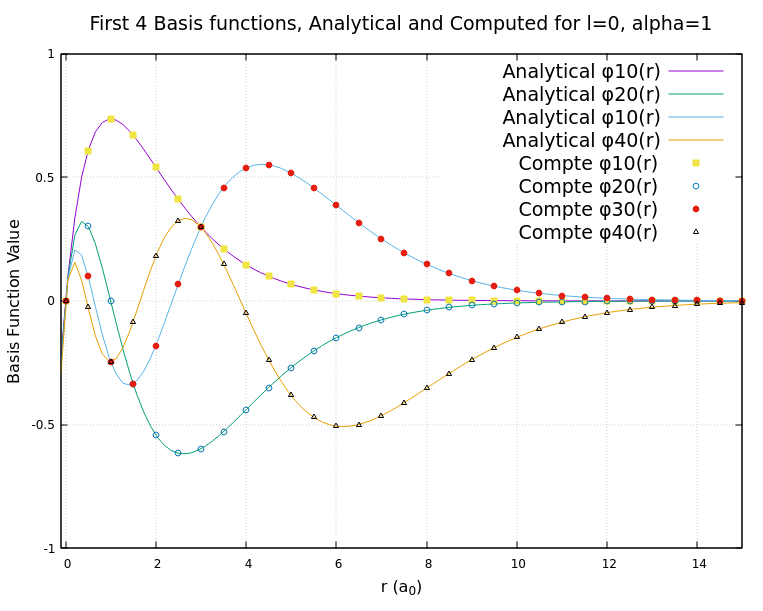
\includegraphics[scale=0.62]{Images/l0a1.png}\\
    	\caption{First four analytical Laguerre basis functions vs discrete computational Laguerre basis functions, for l=0, $\alpha$=1}
    	\label{l0a1}
    \end{figure}
    \begin{figure}[H]
    	\centering
    	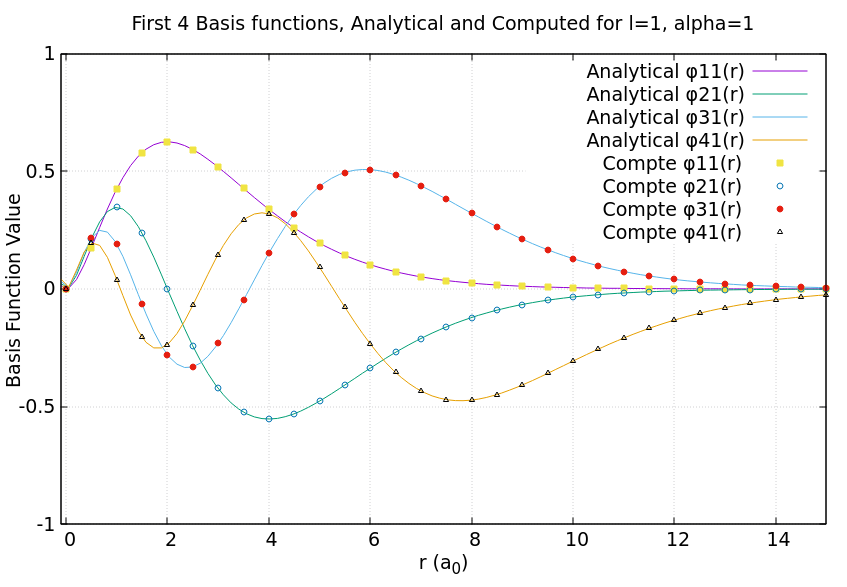
\includegraphics[scale=0.62]{Images/l1a1.png}\\
    	\caption{First four analytical Laguerre basis functions vs discrete computational Laguerre basis functions, for l=1, $\alpha$=1}
    	\label{l1a1}
    \end{figure}
    \begin{figure}[H]
    	\centering
    	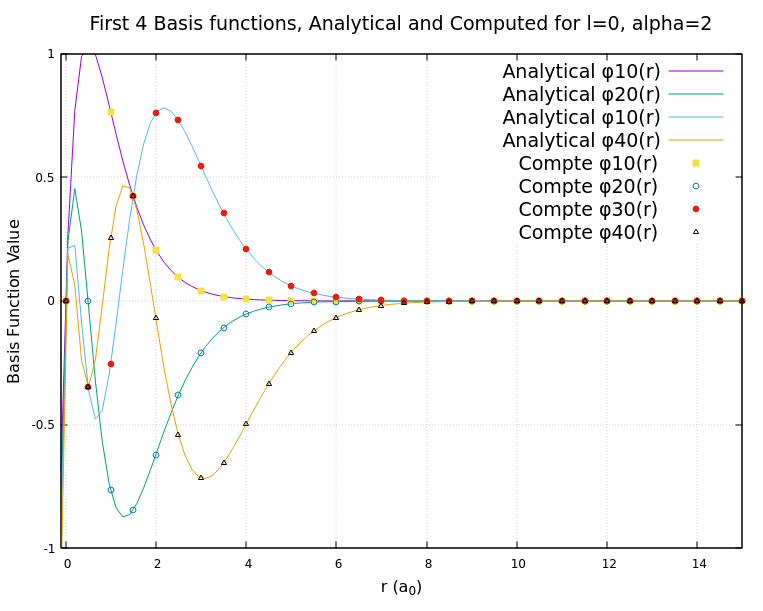
\includegraphics[scale=0.62]{Images/l0a2.png}\\
    	\caption{First four analytical Laguerre basis functions vs discrete computational Laguerre basis functions, for l=0, $\alpha$=2}
    	\label{l0a2}
    \end{figure}
    \begin{figure}[H]
    	\centering
    	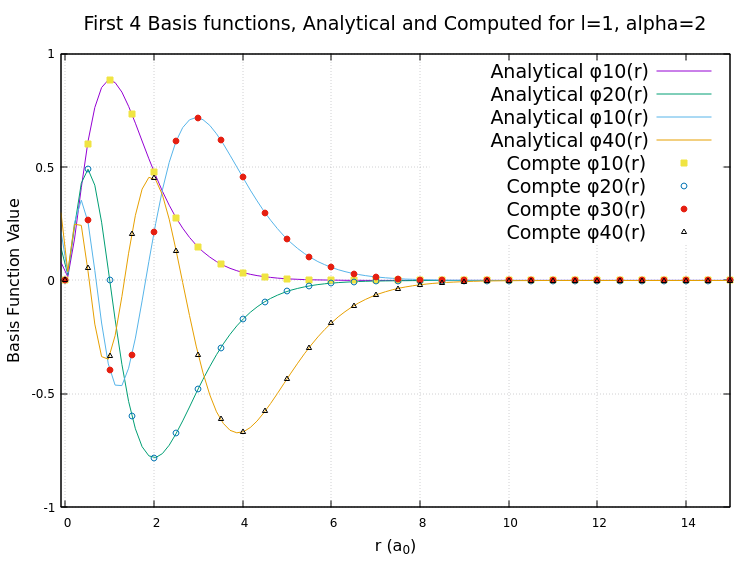
\includegraphics[scale=0.62]{Images/l1a2.png}\\
    	\caption{First four analytical Laguerre basis functions vs discrete computational Laguerre basis functions, for l=1, $\alpha$=2}
    	\label{l1a2}
    \end{figure}
    
    Increasing $\alpha$ decreases the range of the basis functions such that they asymptotically decay to zero faster, expected as all of the functions $\propto e^{-\alpha r}$ (compare figures \ref{l0a1} and \ref{l0a2}). Increasing $l$ for constant $\alpha$ results in a suppression of the wavefunction at the origin (see figures \ref{l0a1}, \ref{l0a2} vs \ref{l1a1}, \ref{l1a2}). The $\alpha$ parameter may produce more for lower N depending on the energy states of interest, if it allows the basis functions to more quickly approximate the fall-off of the true wavefunction. Similar could be said for smaller alpha. In all cases we see a perfect agreement  between the analytical basis functions and the vectorised basis stored in the array.
    
    
    
    
    
    
    \subsection{Problem 3}
    
    
    Section \ref{problem 1} mentions that the radial component of the Hydrogen wavefunction can be determined by the infinite sum of the appropriate Laguerre based basis functions:
    \large
    \begin{gather}
    	\ket{\Phi} = \sum_{j}c_j\ket{\phi_j}
    \end{gather}
    \normalsize
    
    If we make this substitution into the Schrodinger equation:
    \large
    \begin{gather}
    	\sum_{j}c_j\vec{H}\ket{\phi_j} = E\sum_{j}c_j\ket{\phi_j}\\
    	\sum_{j}c_j\bra{\phi_i}\vec{H}\ket{\phi_j} = E\sum_{j}c_j\bra{\phi_i}\ket{\phi_j}
    \end{gather}
    \normalsize
    
    As a matrix equation then becomes:
    \large
    \begin{gather}
    	\sum_{j}c_{ji}\vec{H_{ij}} = E_i\sum_{j}\vec{B_{ij}}c_{ji}
    \end{gather}
    \normalsize


    Close approximations to the true Schrodinger equation solution can be determined for a finite sum, up to some limit of the N'th basis function:
    
	\large
	\begin{gather}
		\sum_{j}^{N}c_{ji}\vec{H_{ij}} = E_i\sum_{j}^{N}\vec{B_{ij}}c_{ji}
	\end{gather}
	\normalsize
	
	As we increase N, functions in the basis ,we will get higher accuracy to the true functions. 
	
	In \textit{main.f90} the provided \textit{rsh.f} function is used to solve this problem, and get approximations to the bound and continuum state hydrogen energy levels and recover the coefficients $c_{ij}$ which can be used in the finite sum:
	\large
	\begin{gather}
		\Phi(r) = \sum_{j}^{N} c_{ji} \phi_j(r)
	\end{gather}
 	\normalsize
 	
 	To recover the radial wavefunctions.
 	
 	To do this, the following definitions of $\vec{H}, \vec{B_{ij}}$ were used:
 	
	\large
	\begin{center}
		\begin{tabular}{cc}
		$\vec{H_{ij}} =$ 	& $ \alpha_{l_i}^2\delta_{ij}    - \frac{\alpha_{l_i}}{(k_i + l_i)}\delta_{ij} -  \frac{\alpha_{l_i}^2}{2}\braket{\phi_{k_il_i}}{\phi_{k_jl_i}} \delta_{l_il_j} \delta_{m_im_j}$ \\
		& \\
		$\vec{B_{ij}} =$	& $\braket{\phi_{k_il_i}}{\phi_{k_jl_i}} \delta_{l_il_j} \delta_{m_im_j}$\\
		\end{tabular}
	\end{center}
	\normalsize
	
	Where we also employ the useful definition:
	\large
	\begin{gather}
		\braket{\phi_{k_il}}{\phi_{k_jl}} = -0.5\sqrt{1-\frac{l(l+1)}{(k_i+l)(k_i+l+1)}}
	\end{gather}
	\normalsize
	
	The code implementation of the calculation of the Hamiltonian and overlap matricies, as well as the use of the rsg function is given below. This is a section of code extracted from \textit{main.f90}, with some definitions removed for brevity, but all can be found in the code repository. 
	
\begin{lstlisting}[language=fortran]
	
... See previous code listing for code prior to this

!use recurrence relation to compute the basis functions
CALL LaguerreSub(alpha, l, nr, N, rgrid, basis)

!implement normalisation condition using simplified factorial
do i = 1, N
	p=1.0
	do j = 0, 2*l
		p = p*(i+2*l-j)
		Print *, p, j
	end do
	normalise = sqrt(alpha /((i+l)* p))
	Print *, "Norm:: ", normalise
	basis(:,i) = normalise*basis(:,i)
end do


!write basis to file for plotting

open(1, file='basisout.txt', action='write')
do i =1,nr
	write(1, '(*(f12.8))'), rgrid(i), basis(i,:)
end do
close(1)

!calculate overlap matrix
B = 0.0d0
do i =1, N-1
	B(i,i) = 1.0d0
	B(i,i+1) = -0.5d0*sqrt(1.0d0-( (l*(l+1.0d0)) / ((i+l)*(i+l+1.0d0))))
	B(i+1,i) = B(i,i+1)
end do
B(N,N) = 1.0d0

!compute H-matrix Elements
H = (-alpha**2/2.0) * B
do i =1,N
	H(i,i) = H(i,i) + alpha**2 - (alpha/(i+l))
end do

Print *, H(i,:)

CALL rsg(N,N,H,B,w,1,z,ier)

!recover wavefunctions:
wf = 0.0d0
do i =1,N
	do j = 1,N
	wf(:,i) = z(j,i)*basis(:,j) + wf(:,i)
	!Print *, wf(:,i)
	end do
end do


open(1, file='wfout.txt', action='write')
do i =1,nr
	write(1, '(*(f12.8))'), rgrid(i), wf(i,:)
end do
close(1)

open(1, file='wout.txt',action='write', access='append')
do i =1,N
	write(1, '(*(f12.8))'), real(N), w(i,1)
end do

... deallocation and end program ...
	
\end{lstlisting}
	
	We have made use of the Kronecker delta functions where they can reduce the number of loop iterations for values of matricies that are always zero. 
	For example, when defining the matrix for the Hamiltonian, we do not need to iterate over the whole thing, we need only add missing components to the diagonal after copying a modified overlap matrix. 
	
	
	From this method we ca show that for $\alpha=1, l=0$, as we increase the nubmer of basis functions, we get a convergence in the Energies of the hydrogen atom to the analytically derived solutions (figures \ref{variedNbound} and \ref{variedNcont})
	
	\begin{figure}[H]
		\centering
		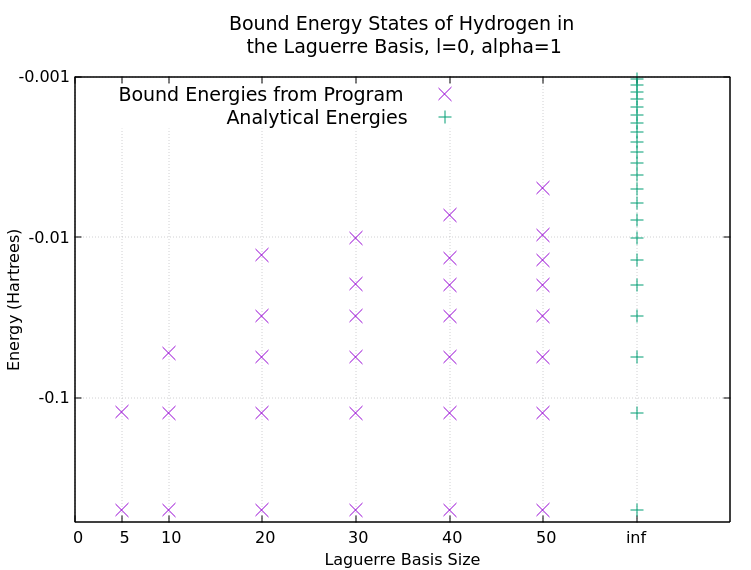
\includegraphics[scale=0.62]{Images/variedN.png}\\
		\caption{For l=0, $\alpha$=1, and increasing N, the predicted bound states of hydrogen energy levels slowly converge to the true analytical distribution.}
		\label{variedNbound}
	\end{figure}
	\begin{figure}[H]
		\centering
		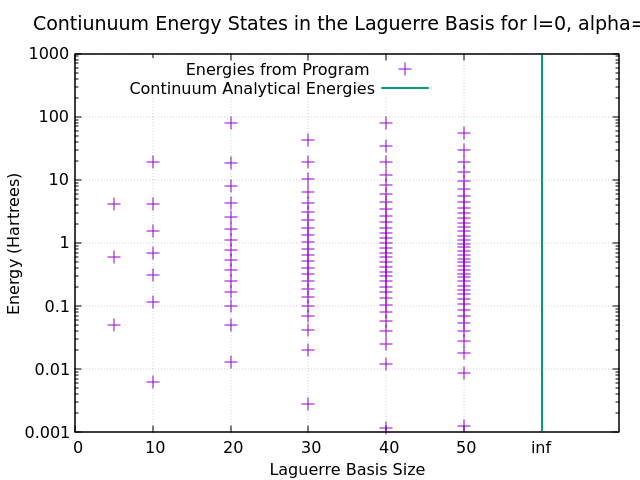
\includegraphics[scale=0.7]{Images/variedNcont.png}\\
		\caption{For l=0, $\alpha$=1, and increasing N, the continuum states of the hydrogen atom slowly tend towards a true continuum.}
		\label{variedNcont}
	\end{figure}
	
	Figures \ref{variedNbound} and \ref{variedNcont} demonstrate the convergence of the bound and continuum state energies for increased basis size. Figure \ref{variedNbound} shows that the bound state predictions for the energies converge to the true values fairly quickly for the lowest energy levels. For the continuum the predictions tend to fill out faster around $E=1$, and very large basis size is would be needed to make a good approximation to the continuum for the lowest energies. 
	
	\begin{figure}[H]
		\centering
		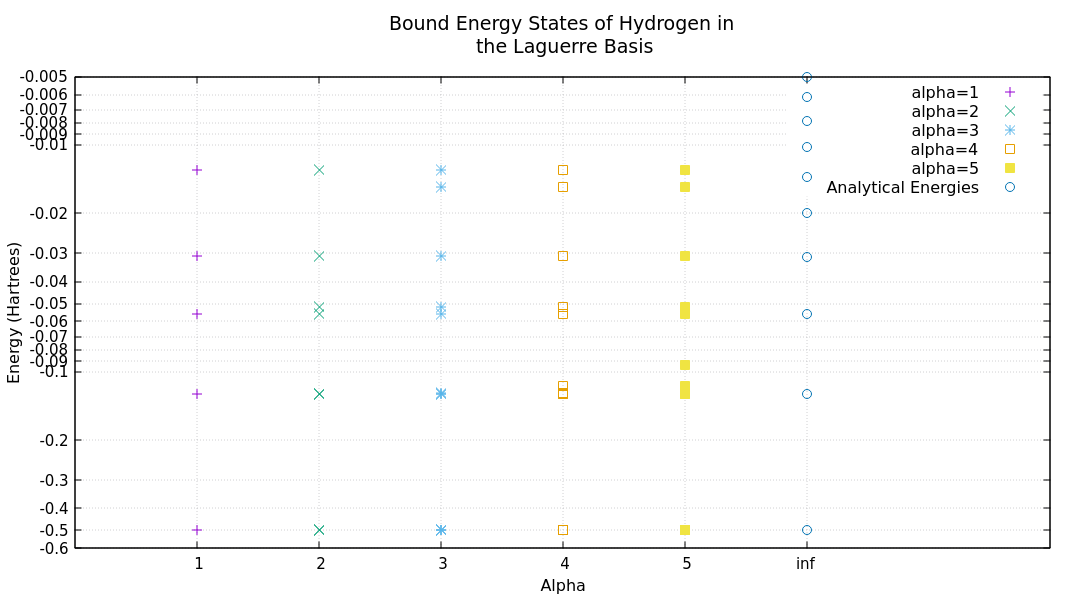
\includegraphics[scale=0.62]{Images/varieda.png}\\
		\caption{N=20 bound states for varied $\alpha$.}
		\label{variedalpha}
	\end{figure}
	\begin{figure}[H]
		\centering
		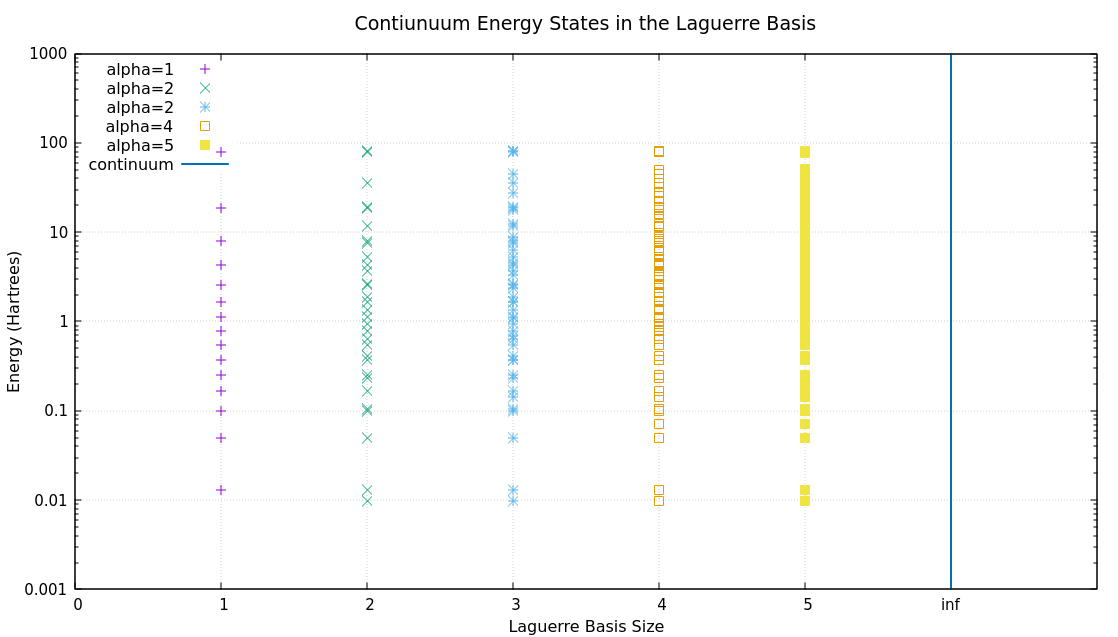
\includegraphics[scale=0.62]{Images/variedacont.png}\\
		\caption{N=20 continuum states for varied $\alpha$.}
		\label{variedalphacont}
	\end{figure}
	
	From figures \ref{variedalpha} and \ref{variedalphacont} the increase in $\alpha$ appears to increase the rate that the continuum states are populated but decreases the accuracy of the bound states. For the bound states and limited N=20, the higher the alpha, the more erroneous bound state energy values there are. The choice of $\alpha$ will strongly influence scattering calculations. For collision where the lowest states are expected to be excited, a small $\alpha$ would converge faster, requiring smaller basis arrays, but for collisions where electrons are expected to enter a continuum state, higher alpha might be preferable because it covers the continuum faster for the same basis size. 
	
	For N=500, we calculate the first three bound state s-wave and p-wave radial wavefunctions using the finite summation of the basis functions with their coefficients, as previously outlined. These calculated wavefunction vectors are compared to the complete analytical solutions in figures \ref{swave} and \ref{pwave}. 
	
	We note high agreement between the analytical and calculated solutions, with a key anomaly. For the s-state solutions, the program returns a 2s wavefunction which is the negative of the normal analytical solution, the same is true for the 2p state. These negative solutions are also true solutions of the Schrodinger equation and deliver the same observable outcomes, due to the fact that observables are associated with the square of the wavefunction. 
	
	\begin{figure}[H]
		\centering
		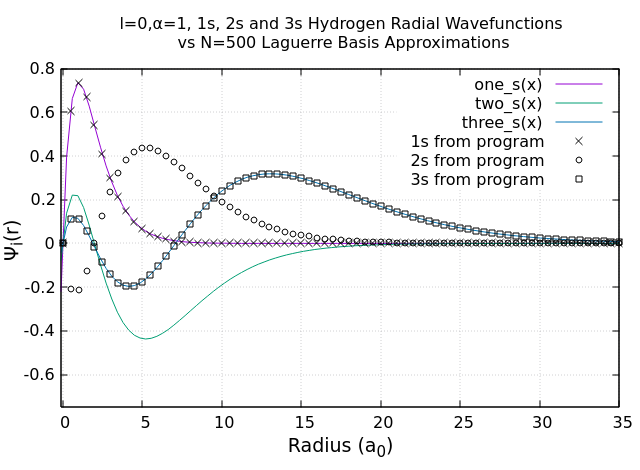
\includegraphics[scale=0.8]{Images/swave.png}\\
		\caption{N=500 first three bound state, s-wave, radial wavefunctions of Hydrogen.}
		\label{swave}
	\end{figure}
	\begin{figure}[H]
		\centering
		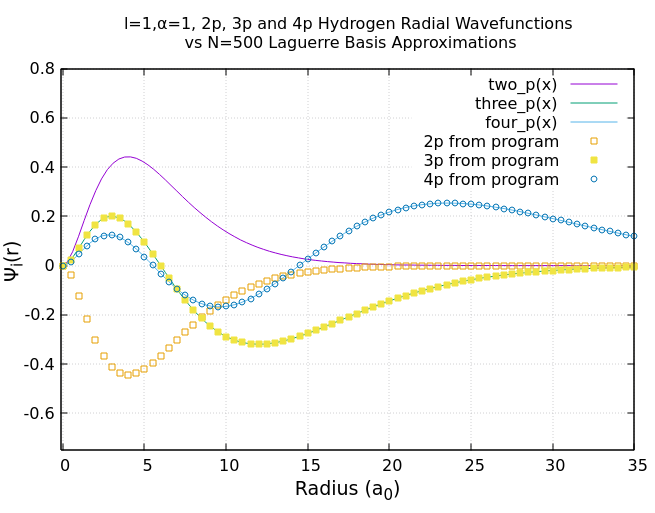
\includegraphics[scale=0.8]{Images/pwave.png}\\
		\caption{N=500 first three bound state, p-wave, radial wavefunctions of Hydrogen.}
		\label{pwave}
	\end{figure}
	
	
	
	
\end{document}












